\documentclass{article}
\usepackage{graphicx} 
\usepackage{amsmath}
\usepackage{amsfonts}
\usepackage[left=1in, right=1in, top=1in, bottom=1in]{geometry}
\usepackage{url}
\usepackage{titlesec}
\usepackage{listings}
\usepackage[hidelinks]{hyperref}
\usepackage{media9}
\usepackage{ocgx2}
\usepackage{comment}

\title{Simulation of Wave Propagation in a Time-modulated Metamaterial}
\author{Mauro Morini}
\date{\today}

\begin{document}
\maketitle

\tableofcontents
\newpage
\section{Introduction}
The goal of this short project was to simulate the propagation of a plane wave in two dimensions through a wave guide containing time modulated meta-materials functioning as resonators. These resonators slow down the speed of propagation of the wave by time dependant functions $\rho$ and $\kappa$. The idea was to place resonators in the wave guide, such that they obstruct most of the waves path with the exception of a slit. When the wave hits the resonators we expected to see an interference pattern behind the resonators, as well as the interference of the scattered wave onto the incident wave in front of the resonators.

\subsection{The Problem}
We considered a rectangular, two-dimensional domain $\Omega = (0,L_x) \times (0,L_y)$ and a time interval of interest $(0,T)$. The boundary $\partial\Omega$ of $\Omega$ is subdivided into the four sides of the rectangle: \\ \\
$\Gamma_1 = \{(x,y)\in \Omega\, |\, x = 0\}$, 
$\Gamma_2 = \{(x,y)\in \Omega\, |\, y = 0\}$,
$\Gamma_3 = \{(x,y)\in \Omega\, |\, y = L_y\}$,
$\Gamma_4 = \{(x,y)\in \Omega\, |\, x = L_x\}$ \\ \\
We were interested in a solution $u$ of the wave equation with time and space dependent wave speed $c(x,t) = \sqrt{\kappa (x,t)/\rho(x,t)}$. $u$ should satisfy homogeneous Neumann boundary conditions on $\Gamma_i$ for $i = 2,3$ and should be described by a non homogeneous, time dependent Neumann boundary condition on $\Gamma_1$. For $\Gamma_4$ we choose a first-order absorbing boundary condition to imitate an ongoing wave guide and avoid unwanted reflection. This yields the following PDE:
\begin{equation}\label{eq:strong formulation}
\left\{
\begin{aligned}
	\frac{\partial}{\partial t} \Big( \frac{1}{\kappa(x,t)}\frac{\partial}{\partial t}u(x,t)			\Big)-
	\nabla \cdot \Big(\frac{1}{\rho (x,t)}\nabla u(x,t)\Big) = 0, \qquad  &\text{in}					\quad \Omega \times (0,T) \\
	u = u_0, \quad \frac{\partial u}{\partial t} = v_0, \qquad &\text{in}\quad \Omega \times \{0\}\\
	\frac{\partial u}{\partial n} = g(x,t), \qquad &\text{on}\quad \Gamma_1 \times (0,T)\\
	\frac{\partial u}{\partial n} = 0, \qquad &\text{on}\quad \Gamma_i \times (0,T) \qquad
	\text{for}\quad i=2,3\\
	\frac{\partial u}{\partial t}+ c\frac{\partial u}{\partial n}=0, \qquad &\text{on}\quad 		\Gamma_4 \times (0,T)\\
\end{aligned}
\right.
\end{equation}
\subsection{Methodology}
To simulate the plane wave we first had to create a triangulation of the given wave guide using Matlab's \texttt{PDE-Toolbox}. To then approximate the exact solution we used linear finite elements in space and the Leap-Frog method in time as well as some methods to reduce the computational cost. 

\section{Mesh Creation}\label{Mesh Creation}
We created two types of meshes:\\
Firstly an equidistant triangulation of the unit square $\Omega_2 := (0,1)\times (0,1)$ to test our code. For this we used our Matlab function \texttt{generateMesh2dUnitSquare} from \textit{Numerical Methods for PDE}.\\
Then to triangulate our final domain $\Omega = (0,L_x) \times (0,L_y)$ we wrote a function \texttt{gen\_mesh} which outputs a geometry matrix $dl$ containing the necessary information of the mesh using Matlab's function \texttt{decsg} and a coordinate matrix containing the defining vertices of the domain and it's sub-domains (in our case the resonators).\\
We then wrote a script \texttt{generate\_rectangular\_Mesh\_with\_resonators} which creates said geometry matrix $dl$ and introduces the data into a pde model object using the \texttt{generateMesh} command of Matlab. Finally we were able to extract the point, edge and connectivity matrices from the resulting pde model using the \texttt{meshToPet} command. \\
We chose the following variables for the domain $\Omega$:
$L_x = 20$ and $L_y = 10$ and the resonators we placed as rectangles with the following vertices: \\
$R_1$: $x_1 = (12,0), x_2 = (12.25,0), x_3 = (12.25,5.5), x_4 = (12,5.5),$ \\
$R_2$: $x_5 = (12,6), x_6 = (12.25,6), x_7 = (12.25,10), x_8 = (12,10)$.\\ \\

\begin{figure}[h]
\centering
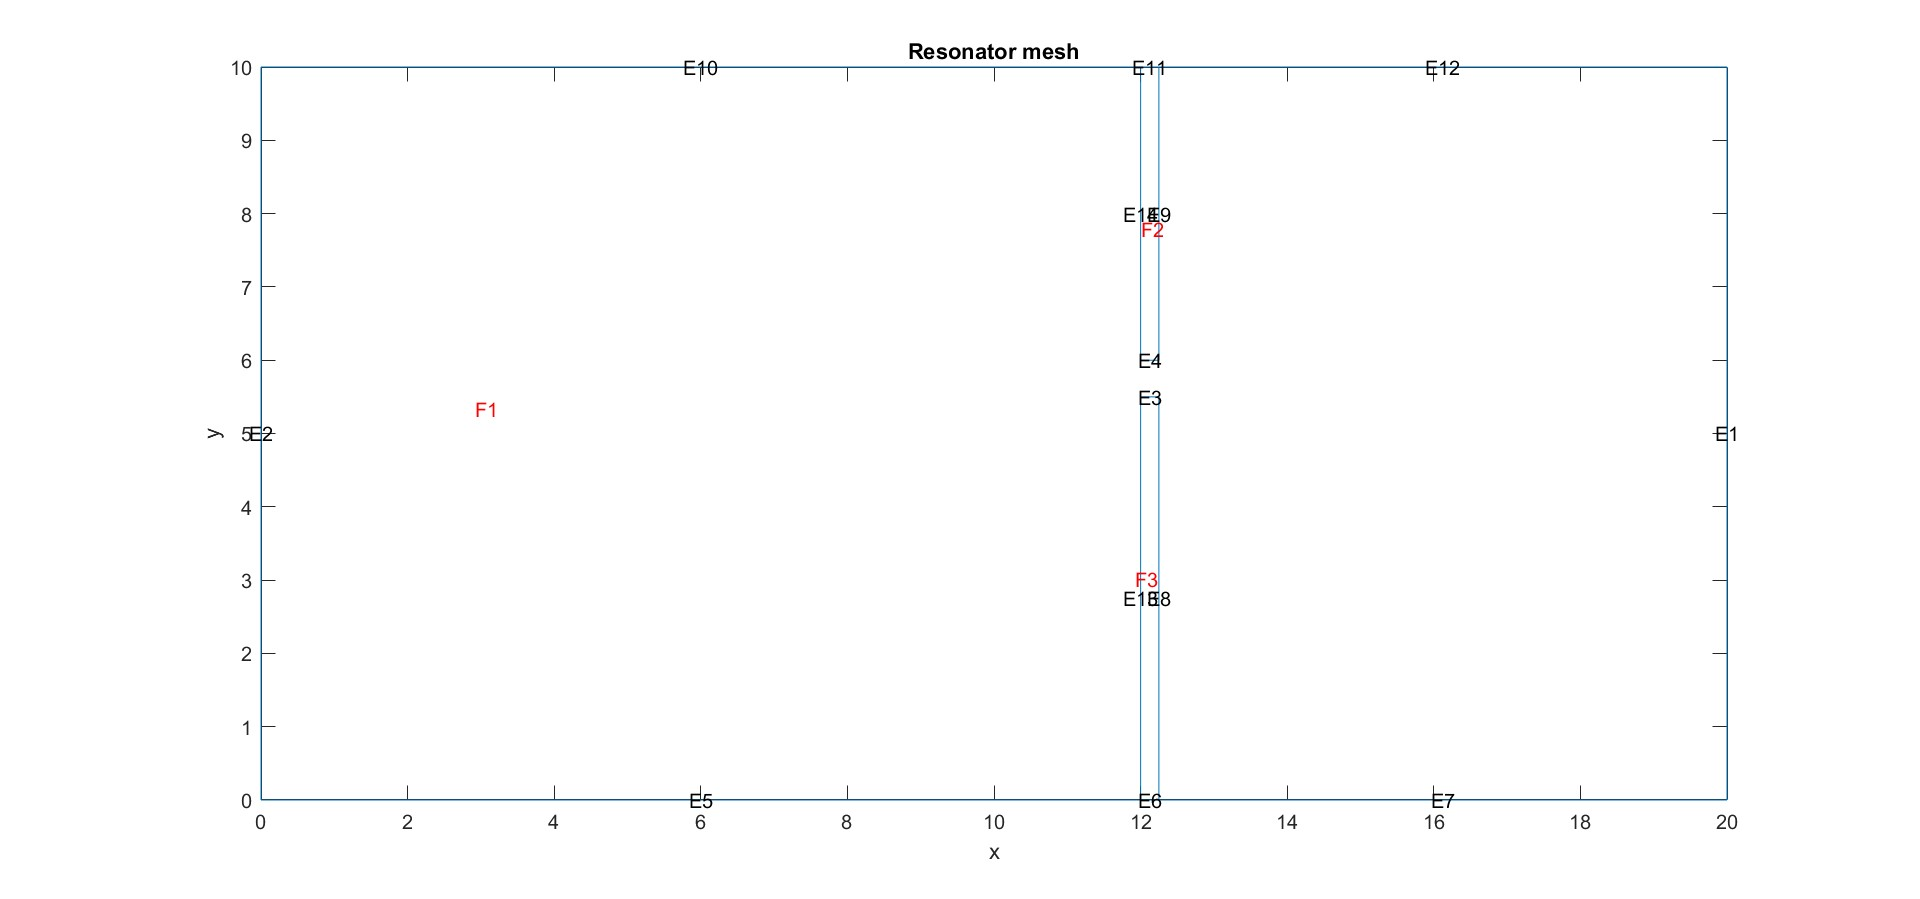
\includegraphics[width = \linewidth]{domain.jpg}
\caption{The domain $\Omega$}
\label{domain}
\end{figure}

In Figure \eqref{domain} we can see the resonators denoted by $F2$ and $F3$ and the background medium by $F1$. \\ \\

Since we expected the important part of our simulation to be happening inside and in the close vicinity of the resonators, we set the mesh size $h = 0.03$ there. On the other hand the in the background medium we expected simpler behaviour of the wave, which is why we chose a general maximal mesh size of $H = 0.5$ on all of $\Omega$. The resulting triangulation can be see in Figure \eqref{triangulation}. For the final simulation we ended up decreasing the maximal mesh size $H = 0.1$ for smoother pictures.

\begin{figure}[h]
\centering
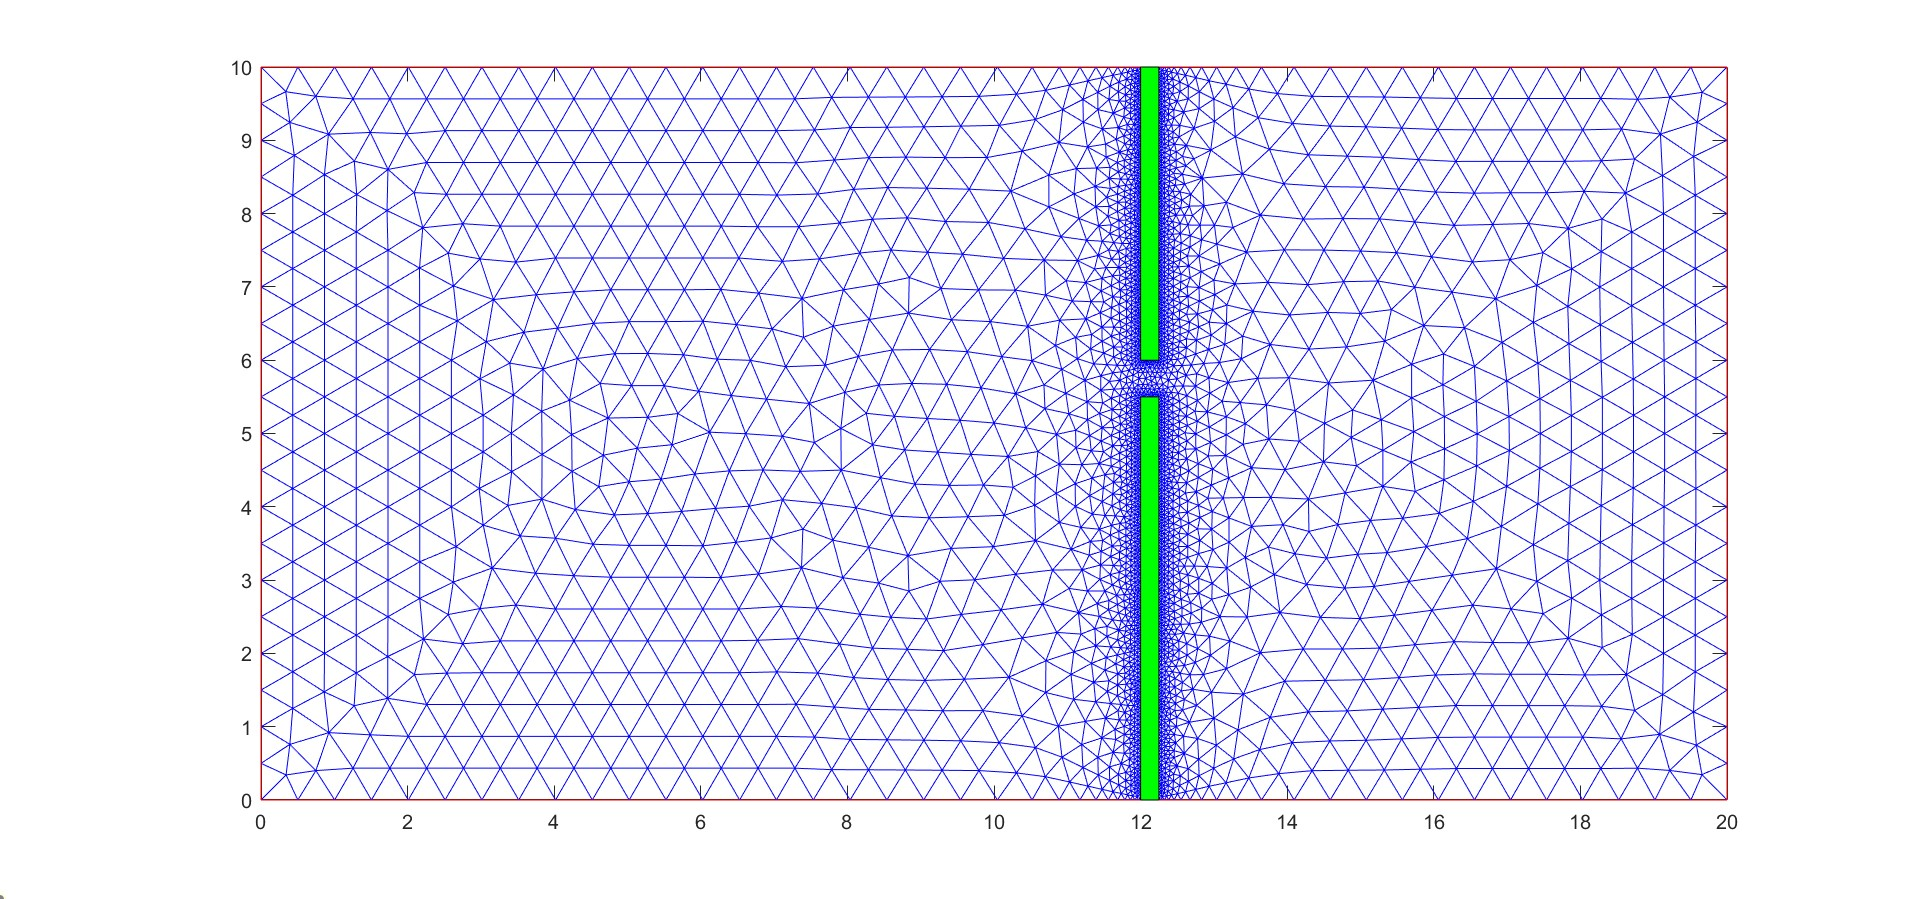
\includegraphics[width = \linewidth]{triangulation.jpg}
\caption{Triangulation of $\Omega$ with $H = 0.5$}
\label{triangulation}
\end{figure}

\section{Numerical Simulation}
\subsection{Time Independent Problem}
First we needed to extend our already existing finite element code for the problem at hand and test our implementation. Firstly we were missing a non homogeneous Neumann boundary condition implementation, so we considered the following elliptical, time independent problem on the unit square $\Omega_2 = (0,1) \times (0,1)$:

\begin{equation}\label{time indep strong formulation}
\left\{
\begin{aligned}
	-\Delta u + u = f \qquad &\text{in} \quad \Omega_2 \\
	\frac{\partial u}{\partial n} = g \qquad &\text{on} \quad \partial\Omega_2 
\end{aligned}
\right.
\end{equation}
To solve this problem with finite elements, we first derived the weak formulation. For that we multiplied by a test function $v \in V := H^1(\Omega_2)$ and integrated over $\Omega_2$:
\[
	\int_{\Omega_2}fv \, \text{d}x = \int_{\Omega_2}-\Delta u v + u v \,\text{d}x
	\overset{I.P.}{=} \int_{\Omega_2}\nabla u \cdot \nabla v + uv \, \text{d}x
	-\int_{\partial\Omega_2} v \frac{\partial u}{\partial n}\, \text{d}s
	= \int_{\Omega_2}\nabla u \cdot \nabla v + uv \, \text{d}x
	-\int_{\partial\Omega_2} v g\, \text{d}s
\]
This gave us the weak formulation: Find $u \in V$, such that
\begin{equation}\label{time indep weak formulation}
\begin{aligned}
a(u,v) &= \ell(v)\qquad  \forall v\in V \\
a(u,v) &:=  \int_{\Omega_2}\nabla u \cdot \nabla v + uv \, \text{d}x \\
\ell(v) & := \int_{\Omega_2} fv \, \text{d}x + \int_{\partial \Omega_2} vg\, ds
\end{aligned}
\end{equation}
Now after applying our standard Galerkin method to our finite element space $V_h = \{v \in C^0(\overline{\Omega}_2)| \, v|_K \in \mathbb{P}^1(K), \, K\in \mathcal{T}_h\}$ where $\mathcal{T}_h$ is a shape regular (in our case equidistant) triangulation of $\Omega_2$, we got the following linear system:

\[
	(A + M)u = L + G
\]
Here $A,M \in  \mathbb{R}^{N \times N}$ are our standard stiffness, mass matrices respectively, to compute those in Matlab we used our old functions \texttt{stiffnessMatrix2D} and \texttt{massMatrix2D}. $L \in \mathbb{R}^N$ is our standard load vector computed by the function \texttt{loadVector2D} we implemented in \textit{Numerical Methods for PDE's}. Finally $G \in \mathbb{R}^N$ is our new Neumann load vector containing the boundary conditions. To assemble this vector in Matlab one needs to iterate over the boundary edges of the mesh and compute one dimensional boundary integrals over each edge affected by the condition\footnote{For more information see: The Finite Element Method by Mats G. Larson and Frederik Bengzon; Chapter 4.6.2}. \\ \\
We chose the exact solution $u(x_1,x_2) = \text{sin}(\pi x_1)\text{sin}(\pi x_2)$. This leads to:

\[
	f = -\Delta u + u = (1 + \pi^2 + \pi^2)\,\text{sin}(\pi x_1)\text{sin}(\pi x_2)
\]

To find $g$ we recall that $\frac{\partial u}{\partial n} = \nabla u \cdot n$, so we get:
\[
g(x_1,x_2) = \left\{
	\begin{aligned}
		-\pi\, \text{cos}(\pi x_1)\text{sin}(\pi x_2),\qquad x_1 = 0 \\
		-\pi\, \text{cos}(\pi x_2)\text{sin}(\pi x_1),\qquad x_2 = 0 \\
		\pi\, \text{cos}(\pi x_1)\text{sin}(\pi x_2),\qquad x_1 = 1 \\
		\pi\, \text{cos}(\pi x_2)\text{sin}(\pi x_1),\qquad x_2 = 1 \\
	\end{aligned}
	\right.
\]

We calculated the numerical solutions and the $L^2$-error for $h = 2^{-i}$, $i = 4,...,7$. \\
To compute the $L^2$-error we used the function \texttt{error2d} we implemented in the course last semester. As expected we observed the error to be decreasing like $\mathcal{O}(h^2)$.

\begin{figure}[!h]
	\begin{minipage}[c]{0.5\linewidth}
		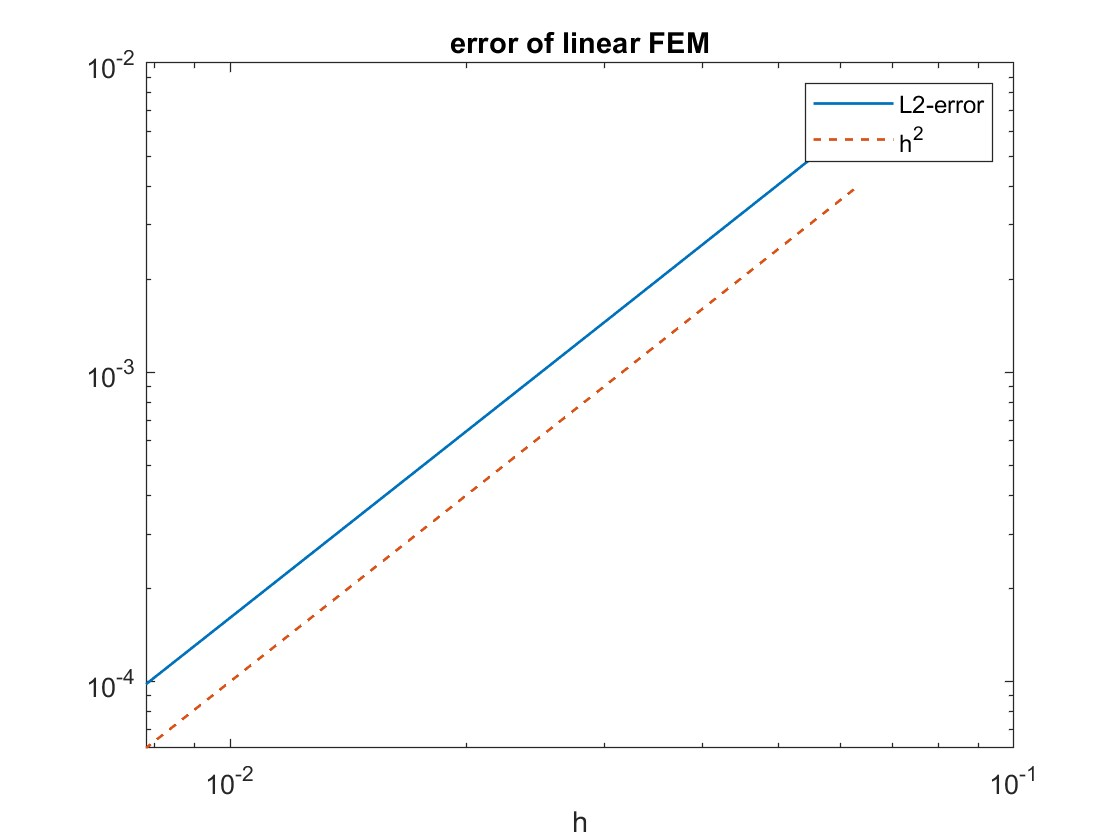
\includegraphics[width=\linewidth]{E2error.jpg}
	\end{minipage}
	\begin{minipage}[c]{0.5\linewidth}
		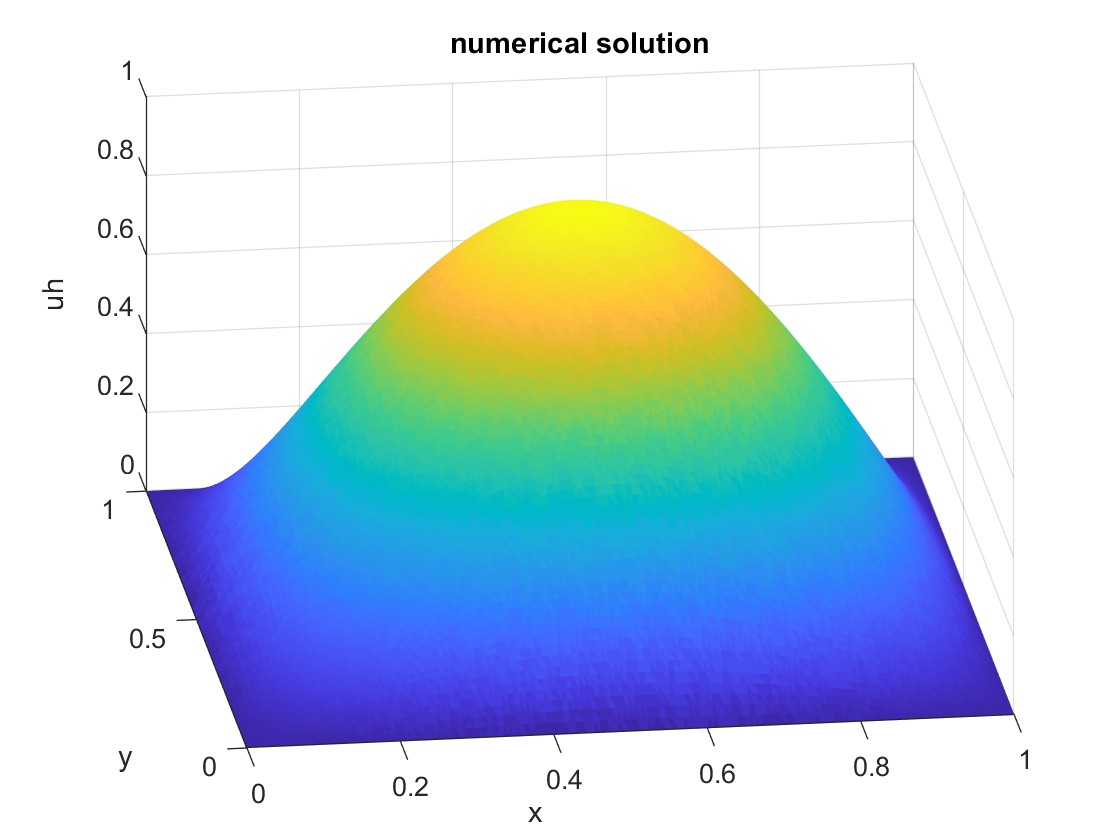
\includegraphics[width=\linewidth]{E2NumSol.jpg}
	\end{minipage}
	\caption{error and plot of $\text{sin}(\pi x_1)\text{sin}(\pi x_2)$}
	\label{fig:E2}
\end{figure}

\subsection{Variational Formulation of the Time Dependent Problem}
After successfully testing our finite element code on a time independent problem, we returned to the time dependent problem \hyperref[eq:strong formulation]{\eqref{eq:strong formulation}}.
To derive the weak formulation we multiplied \hyperref[eq:strong formulation]{\eqref{eq:strong formulation}} by a test function $v\in V := H^1(\Omega \times (0,T))$, integrated over $\Omega$ and used integration by parts:
\begin{align*}
	0 = \int_{\Omega} \frac{\partial}{\partial t}\Big(\frac{1}{\kappa}\frac{\partial u}			{\partial t}\Big)v - \nabla \cdot \Big(\frac{1}{\rho}\nabla u\Big)v\,\text{d}x 					\overset{I.P.}{=}
	\int_{\Omega} \frac{\partial}{\partial t}\Big(\frac{1}{\kappa}								\frac{\partial u}{\partial t}\Big)v + \frac{1}{\rho}\nabla u \cdot \nabla v \, \text{d}x
	- \int_{\partial \Omega} \frac{v}{\rho} \frac{\partial u}{\partial n} \text{d}s
\end{align*}
Then we inserted the boundary conditions into the boundary term:
\[
	\int_{\partial \Omega} \frac{v}{\rho} \frac{\partial u}{\partial n} \text{d}s
	= \int_{\Gamma_1} \frac{v}{\rho} \underbrace{\frac{\partial u}{\partial n}}_{\text{=g}} \text{d}s + 
	\underbrace{\int_{\Gamma_2 \cup \Gamma_3} \frac{v}{\rho} \frac{\partial u}{\partial n} \text{d}s}_{\text{= 0} } + 
	\int_{\Gamma_4} \frac{v}{\rho} \frac{\partial u}{\partial n} \text{d}s
	= \int_{\Gamma_1} \frac{v}{\rho} g\, \text{d}s - 
	\int_{\Gamma_4}\frac{v}{\rho\, c} \frac{\partial u}{\partial t} \, \text{d}s
\]
So finally the weak formulation is: Find $u \in V$, such that:
\begin{equation}\label{eq:weak formulation}
	\begin{aligned}
	a(u,v) &= \ell(v)\qquad  \forall v\in V \\
	a(u,v) &:= \int_{\Omega} \frac{\partial}{\partial t}\Big(\frac{1}{\kappa}
	\frac{\partial u}{\partial t}\Big)v + \frac{1}{\rho}\nabla u \cdot \nabla v \, \text{d}x +
	\int_{\Gamma_4}\frac{v}{\rho\, c} \frac{\partial u}{\partial t} \, \text{d}s\\
	\ell(v) &:= \int_{\Gamma_1} \frac{v}{\rho} g\, \text{d}s 
	\end{aligned}
\end{equation}

\subsection{Galerkin Approximation}
For simplicity we chose $\kappa$ to be time-independent. Let $V_h$ be our linear finite element space in 2D. Then for any fixed time $t \in (0,T)$ we sought a finite element solution of the form: 
\[
	u_h(x,t) = \sum_{i=1}^N u_i(t) \varphi_i(x)
\]
Where $\varphi_i$ are our lagrangian basis functions and the coefficients $u_i$ depend on the time $t$. After applying the standard Galerkin method we get the Galerkin approximation: For a fixed $t\in (0,T)$ find $u_h(t) \in V_h$ such that: 

\begin{gather*}
	a(\sum_{j=1}^N u_j(t)\varphi_j, \varphi_i) = \ell(\varphi_i) \qquad i = 1,..,N \\
	\Leftrightarrow	\sum_{j=1}^N\frac{\partial^2}{\partial t^2} u_j(t) 
	\int_{\Omega}\frac{1}{\kappa}\varphi_j \varphi_i \, \text{d}x + 
	\sum_{j=1}^N u_j(t) \int_{\Omega}\frac{1}{\rho}\nabla\varphi_j \cdot \nabla \varphi_i \, \text{d}x+
	\sum_{j=1}^N\frac{\partial}{\partial t} u_j(t)\int_{\Gamma_4}
	\frac{1}{\rho\, c} \varphi_j \varphi_i \, \text{d}s
	= \int_{\Gamma_1} \frac{1}{\rho} \varphi_i g\, \text{d}s 
	\qquad i = 1,..,N \\
\end{gather*}
By considering element wise contributions we derive the linear system:

\begin{equation}\label{time dep linear system}
	M\ddot{u}(t) + A(t) u(t) + R(t) \dot{u}(t) = G(t)
\end{equation}
$M$ here is our normal mass matrix, but now it is dependent on $\kappa$. This dependency required not much adaptation in our code, since we are working with linear finite elements one can use the \textit{midpoint quadrature rule} to approximate the integral of the product. Similarly $A$ is our stiffness matrix which needed to be adapted to incorporate the scaling by $1/\rho$. $G$ is the previously implemented Neumann load vector, which here takes $g/\rho$ as an input. $R$ is a newly implemented Neumann mass matrix. To assemble $R$ one proceeds exactly as one would assembling a regular mass matrix, but in this case the integrals that are to be computed are not element wise, but rather boundary edge wise\footnote{For more information see: The Finite Element Method by Mats G. Larson and Frederik Bengzon; Chapter 4.6.2}. These edge wise integrals are line integrals in one dimension, hence the assembly of  $R$ is analogous to the 1D assembly of the mass matrix. The code for it can be found in \texttt{neumannMassMatrix2D}.
\subsection{Time Discretization}
To discretize in time we used Leap Frog for the second order derivative and a centred difference quotient for the first order derivative in time. Fix $\Delta t > 0$ and let $u^m = u(t_m) = u(m \Delta t)$ denote the finite element vector at a fixed time $t_m \in (0,T)$, then we got the following two step scheme in time from \eqref{time dep linear system}:
\begin{equation}\label{fully discrete scheme}
\begin{aligned}
	M\Big(\frac{u^{m+1} - 2u^m +u^{m-1}}{\Delta t^2}\Big) + 
	A(t_m)u^m + R(t_m)\Big(\frac{u^{m+1}-u^{m-1}}{2\Delta t}\Big) = G(t_m) \\
	\Leftrightarrow \Big(\frac{1}{\Delta t^2} M + \frac{1}{2\Delta t} R(t_m)\Big)u^{m+1} = 	
	G(t_m) + \Big(\frac{2}{\Delta t^2} M - A(t_m)\Big)u^m - 
	\Big(\frac{1}{\Delta t^2}M - \frac{1}{2\Delta t}R(t_m)\Big)u^{m-1}
\end{aligned}
\end{equation}
From the initial conditions $u^0 = u_0$ is given, so we needed to compute an approximation of $u^1$ using the second initial condition $\partial_t u^0 = v_0$. To do so we approximate $\partial_t u^0$ by a centred difference quotient implementing a \textit{ghost point} $u^{-1}$:
\begin{align*}
	v_0 = \frac{\partial u}{\partial t} \approx \frac{u^1 - u^{-1}}{2\Delta t} \qquad
	\Leftrightarrow \qquad u^-1 \approx u^1 - 2\Delta t v_0
\end{align*}
Plugging this into our fully discrete scheme \eqref{fully discrete scheme} for $m=0$ gives us a formula for $u^1$. From there on we continue iteratively. 
\subsection{Time Discretization Test}
Next we wanted to test our fully discrete scheme. To do so we considered the domain $\Omega_2$ the unit square without any resonators, in particular we set $c \equiv \kappa \equiv \rho \equiv 1$ on all of $\Omega_2$. We chose the exact solution to be $u(x_1,x_2,t) = \text{cos}(\pi(x_1-t))/\pi$, this lead  to:
\begin{equation*}
\left\{
	\begin{aligned}
		u_0(x_1,x_2) = u(x_1,x_2,0) &= \frac{\text{cos}(\pi x_1)}{\pi} \\
		v_0(x_1,x_2) = \frac{\partial u}{\partial t}(x_1,x_2,0) &= \text{sin}(\pi x_1) \\
		g(x_1,x_2,t) = \nabla u \cdot (-1,0)^T &= \text{sin}(\pi (x_1 - t))
	\end{aligned}
	\right.
\end{equation*}
We set $T = 1$, $h = 2^{-i}$, for $i = 3,..,7$ and $\Delta t = r h$ with $r = 0.5$, calculated the $L^2$-error for each mesh size $h$ and plotted the numerical solution on the finest mesh at the times $t = 0.25, 0.5, 0.75, 1$ in Figure \eqref{fig:E3}

\begin{figure}[!h]
	\begin{minipage}[c]{0.5\linewidth}
		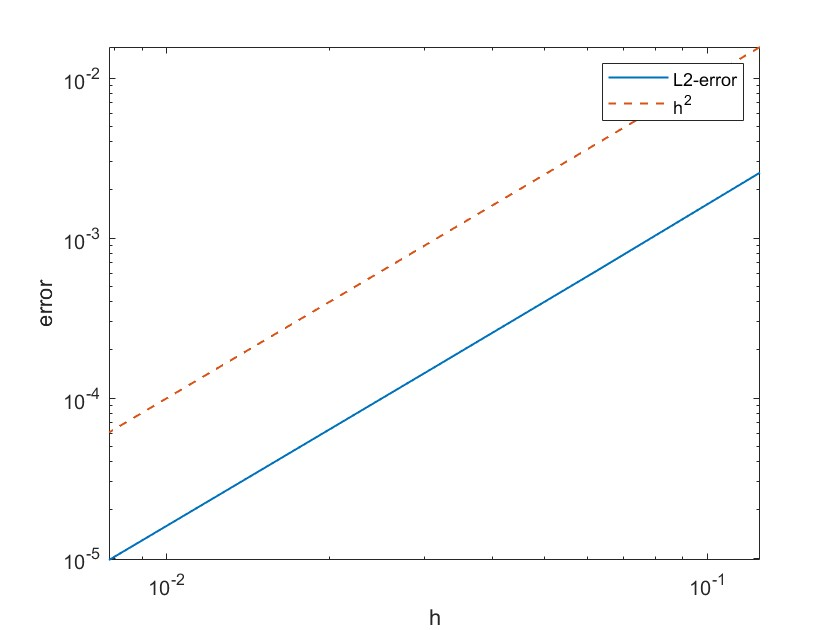
\includegraphics[width=\linewidth]{E3error.jpg}
	\end{minipage}
	\begin{minipage}[c]{0.5\linewidth}
		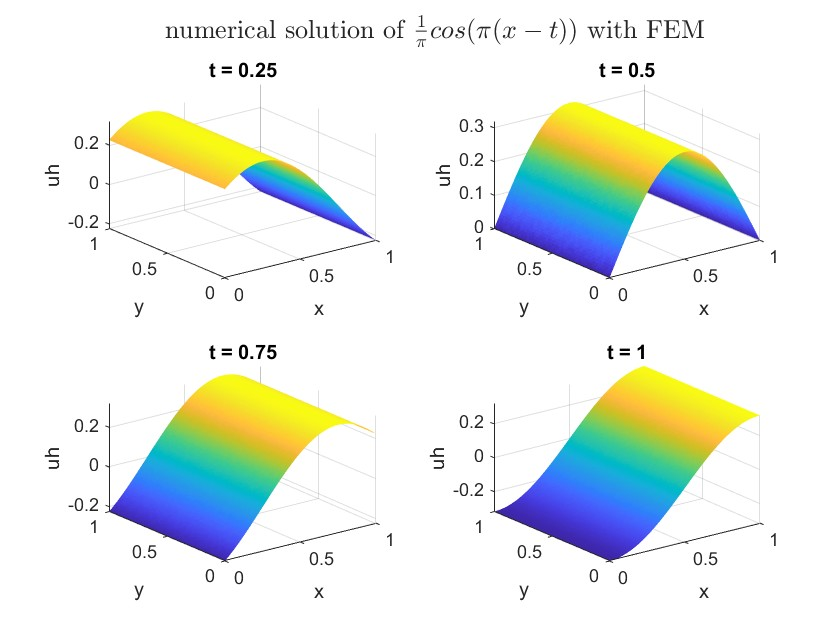
\includegraphics[width=\linewidth]{E3NumSol.jpg}
	\end{minipage}
	\caption{error and plot of $\text{cos}(\pi(x_1-t))/\pi$ }
	\label{fig:E3}
\end{figure}

\subsection{Simulation with Resonators}
After successfully testing our implementation we were then able to apply our code to the mesh we created in section \ref{Mesh Creation}. We define:
\begin{equation*}
\kappa(x,t) = 
\left\{
\begin{aligned}
1, \qquad x\notin R_i \\
0.2, \qquad x \in R_i
\end{aligned}
\right. ,\qquad
\rho(x,t) = 
\left\{
\begin{aligned}
1, \qquad x\notin R_i \\
\rho_r(t), \qquad x \in R_i
\end{aligned}
\right.
\end{equation*}
for $i = 1,2$ with 
\[
	\rho_r(t) = \frac{0.1}{1 + 0.2\, \text{cos}(t\pi/2)}
\]
For the non homogeneous Neumann boundary condition we used: 
\[
	g(x_1,x_2,t) = \text{sin}(\omega(x_1-t)) \qquad \forall\, x_2 
	\in (0,L_y)
\]
Where $\omega = 2\pi$. And we used homogeneous initial conditions
$u_0 \equiv v_0 \equiv 0$. We calculated the numerical solution for different times in $(0,30)$. As expected the wave propagates very regularly until it hits the resonators, because of the slit which allows a portion of the wave to propagate considerably faster than the rest we can observe the interference behind the resonator. On the other hand the resonators slow down the majority of the wave, which leads to the creation of a scattering wave in the opposite direction of the incident wave. These interference patterns can be observed in Figure \eqref{fig:interference}

\begin{figure}
\center
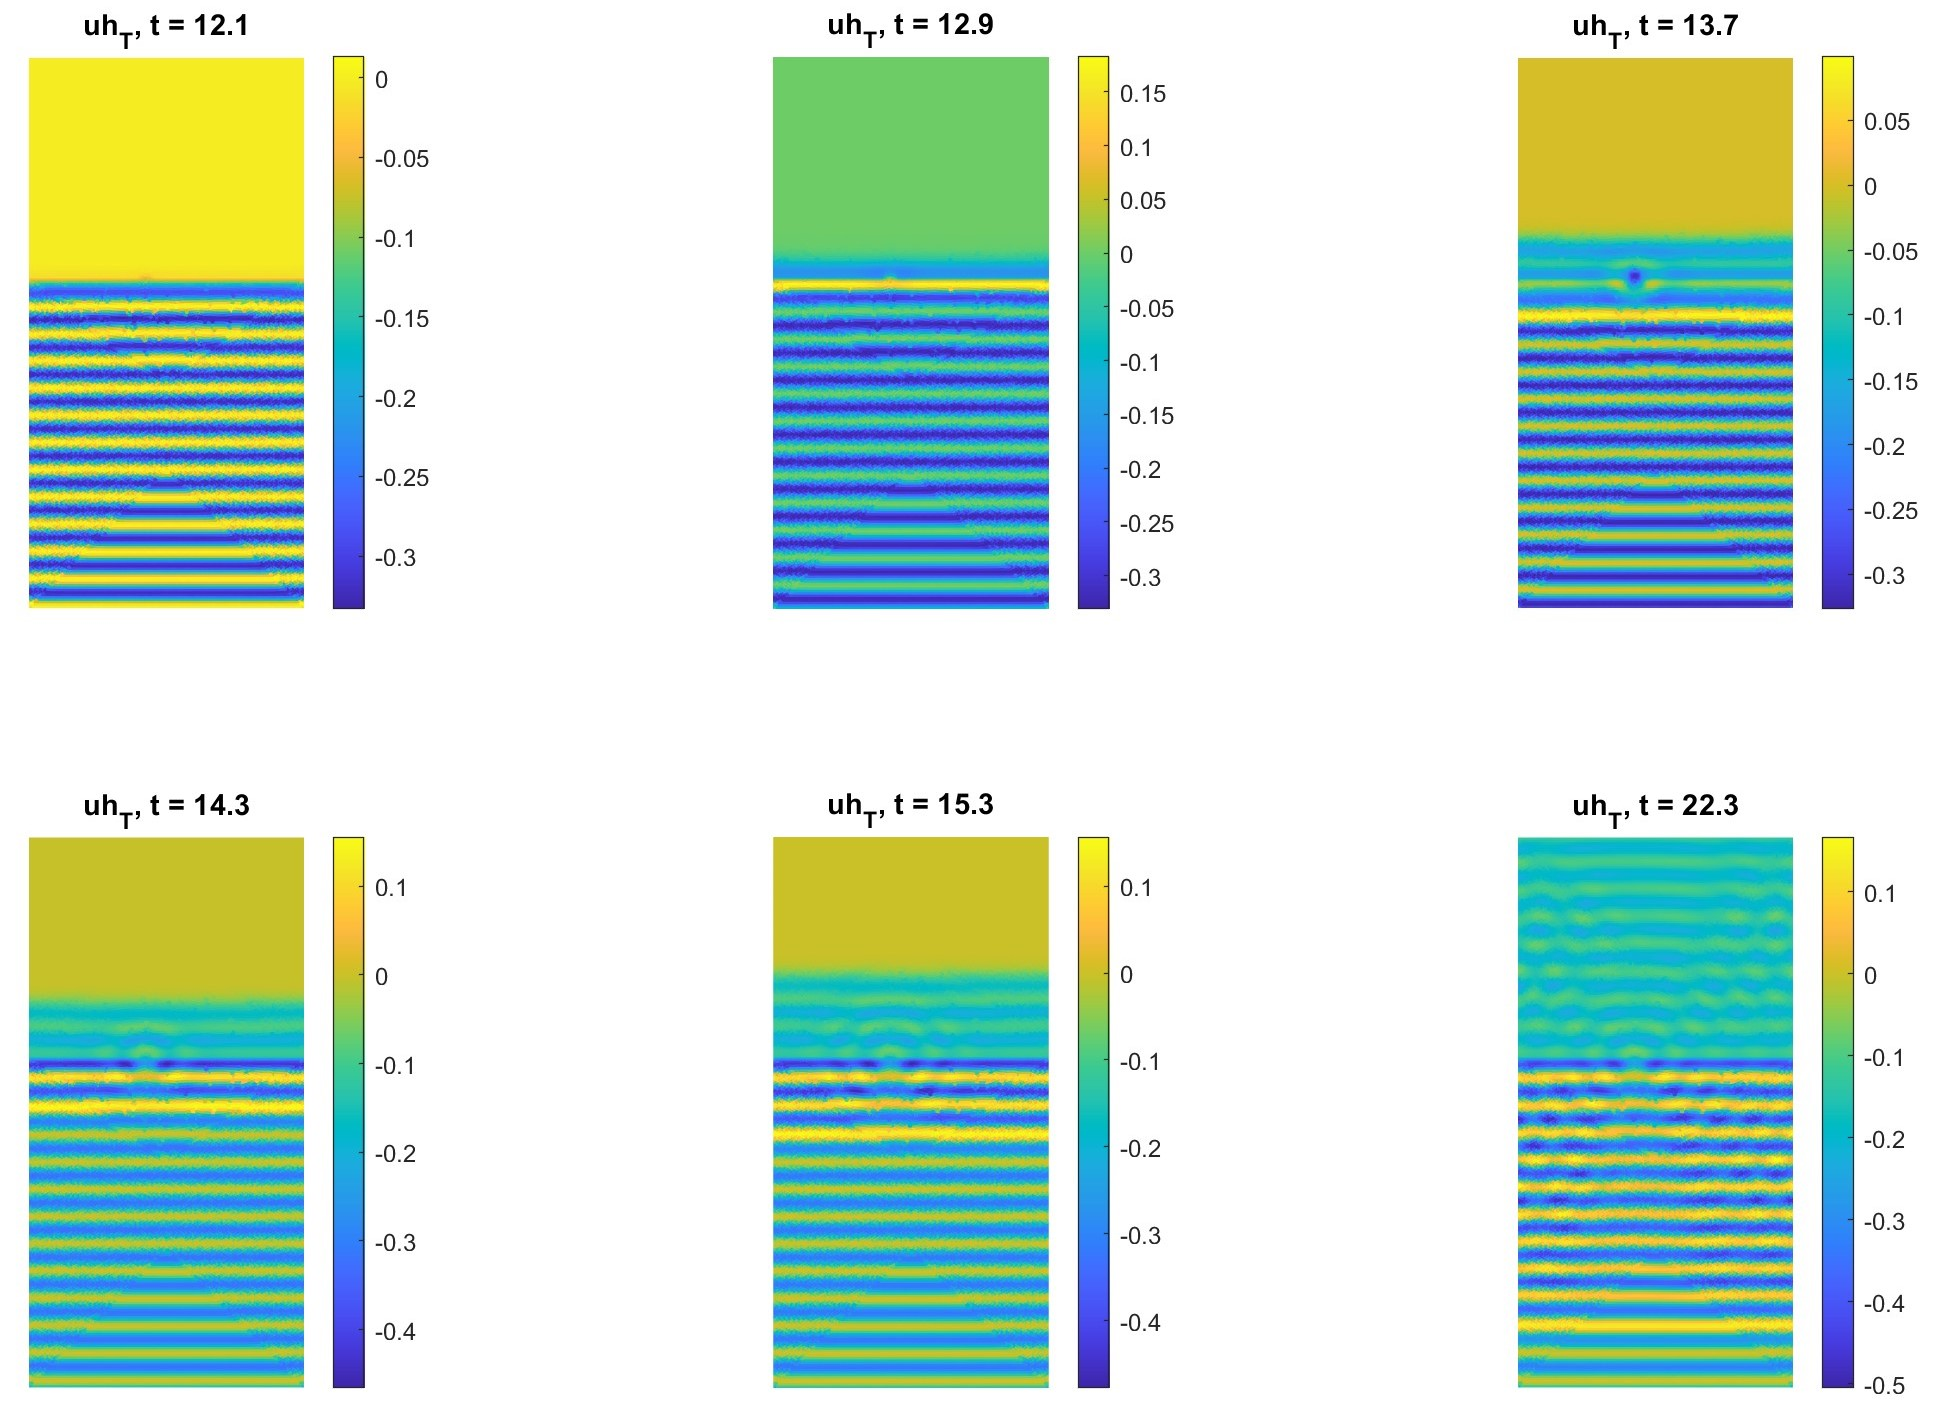
\includegraphics[width=1.05\linewidth]{interferenceBig.jpg}
\caption{Interference pattern on resonator mesh}
\label{fig:interference}
\end{figure}

\subsection{Runtime Improvements}
In the time dependent simulation we did not only have to solve a very big system of equations every time step but also assemble the time dependent stiffness matrix for each time. This turned out to be impossibly costly so we did two modifications which reduced the computational load drastically: \\
\subsubsection*{1. Isolating Time Dependence}
Firstly we noted that although $R$ is theoretically time dependent, in reality it is the matrix describing the absorbing boundary condition at the boundary $\Gamma_4$ and therefore only influenced by values at $\Gamma_4$, i.e.
\begin{align*}
	&\kappa(x,t) = \rho(x,t) = c(x,t) = 1\qquad &\forall 
	x \in \Gamma_4, t \in (0,T) \\
	\Rightarrow &R(t_m) = R(0) = R \qquad &\forall m\geq 0.
\end{align*}
Secondly we noted that both $\kappa$ and $\rho$ are piecewise constant in space. So we got:
\begin{align*}
 	\int_{\Omega} \frac{1}{\rho} \nabla \varphi_j 
 	\cdot \nabla \varphi_i \,\text{d}x &=
 	\int_{R_1 \cup R_2} \frac{1}{\rho} \nabla \varphi_j 
 	\cdot \nabla \varphi_i \,\text{d}x +
 	\int_{\Omega\setminus R_1 \cup R_2} \frac{1}{\rho} 
 	\nabla \varphi_j 
 	\cdot \nabla \varphi_i \,\text{d}x \\ 	
 	&=
 	\frac{1}{\rho}\int_{R_1 \cup R_2} \nabla \varphi_j 
 	\cdot \nabla \varphi_i \,\text{d}x +
 	\int_{\Omega\setminus R_1 \cup R_2}
 	\nabla \varphi_j 
 	\cdot \nabla \varphi_i \,\text{d}x  	\\
\end{align*}
This meant that we could separately assemble a background material stiffness matrix $A_{\text{backg}}\in \mathbb{R}^{N\times N}$ and a resonator stiffness matrix $A_{\text{res}}\in \mathbb{R}^{N\times N}$ which only consider the elements outside or inside the resonators respectively. Finally it holds that:
\[
	A(t) = A_{\text{backg}} + \frac{1}{\rho (x,t)} A_{\text{res}}
	\qquad \forall t \in (0,T)
\]
where  $x \in R_1  \cup R_2$ arbitrary. \\
Therefore we only had to assemble the stiffness matrix once at the beginning and only had to multiply the factor $1/\rho$ in each time step

\subsubsection*{2. Mass Lumping:}
To simplify the system \eqref{fully discrete scheme} (which we need to solve in each time step) we used the technique of \emph{Mass Lumping}. Since both $M$ and $R$ are forms of mass matrices we could \emph{lump} the element wise contributions onto the diagonal entries of the respective matrix, to do so we created diagonal matrices $M_{\text{lump}},R_{\text{lump}}$ where each diagonal entry corresponds to the sum of the row elements in $M,R$. So we defined:
\[
	M_{\text{lump}} := \text{diag}\Big(\sum_{j=1}^N M_{1,j},..,
	\sum_{j=1}^N M_{N,j}\Big), \qquad
	R_{\text{lump}} := \text{diag}\Big(\sum_{j=1}^N R_{1,j},..,
	\sum_{j=1}^N R_{N,j}\Big)	
\]
and exchanged $M_{\text{lump}},R_{\text{lump}} \leftrightarrow M,R$. \\
This makes inverting the matrix $(M_{\text{lump}}/\Delta t^2 + R_{\text{lump}}/(2 \Delta t))$, and hence solving the system a lot cheaper.

\begin{comment}

\subsection{Movie}
\includemedia[
  width=0.6\linewidth,
  height=0.45\linewidth,
  activate=pageopen,
  addresource=spacy wave animation.mp4,
  flashvars={source=spacy wave animation.mp4}
]{}{VPlayer.swf}
\end{comment}

\newpage
\section{References}
\begin{enumerate}
\item Prof. Dr. Marcus J. Grote. \textit{Numerical Methods for Partial Differential Equations}. Fall Semester, 2023
\item Prof. Dr. Marcus J. Grote. \textit{Numerical Methods for Wave Propagation}. Spring Semester, 2024
\item Larson, G., Mats; Bengzon, Fredrik. \textit{The Finite Element Method: Theory, Implementation and Applications}. Springer.
\end{enumerate}

\newpage
\section{Matlab Code}
\subsection{Scripts}
\subsubsection{generate\_rectangular\_Mesh\_with\_resonators}
\lstinputlisting[language=Matlab]{../code/generate\_rectangular\_Mesh\_with\_resonators.m}

\subsubsection{NMWP\_Project\_E2}
\lstinputlisting[language=Matlab]{../code/NMWP\_Project\_E2.m}

\subsubsection{NMWP\_Project\_E3}
\lstinputlisting[language=Matlab]{../code/NMWP\_Project\_E3.m}

\subsubsection{NMWP\_Project\_E4}
\lstinputlisting[language=Matlab]{../code/NMWP\_Project\_E4.m}

\subsection{Functions}
% PDE solver
\subsubsection{stiffnessMatrix2D}
\lstinputlisting[language=Matlab]{\detokenize{../code/stiffnessMatrix2D.m}}

\subsubsection{massMatrix2D}
\lstinputlisting[language=Matlab]{../code/massMatrix2D.m}

\subsubsection{loadVector2D}
\lstinputlisting[language=Matlab]{../code/loadVector2D.m}

\subsubsection{neumannMassMatrix2D}
\lstinputlisting[language=Matlab]{../code/neumannMassMatrix2D.m}

\subsubsection{neumannLoadVector2D}
\lstinputlisting[language=Matlab]{../code/neumannLoadVector2D.m}

\subsubsection{waveEqLF2D}
\lstinputlisting[language=Matlab]{../code/waveEqLF2D.m}

\subsubsection{solve\_elliptic\_BVP\_2d\_FEM\_Neumann}
\lstinputlisting[language=Matlab]{../code/solve\_elliptic\_BVP\_2d\_FEM\_Neumann.m}

\subsubsection{error2d}
\lstinputlisting[language=Matlab]{../code/error2d.m}

\subsubsection{gen\_mesh}
\lstinputlisting[language=Matlab]{\detokenize{../code/gen\_mesh.m}}

\subsubsection{triangulation2d}
\lstinputlisting[language=Matlab]{\detokenize{../code/triangulation2d.m}}

\subsubsection{generateMesh2dUnitSquare}
\lstinputlisting[language=Matlab]{\detokenize{../code/generateMesh2dUnitSquare.m}}




\end{document}